\documentclass[a4paper,12pt]{article}  % TODO explain different classes

\usepackage[T1]{fontenc}
\usepackage[utf8]{inputenc}

\usepackage{amssymb, amsmath, amsthm}
\usepackage[output-decimal-marker={,},
            group-separator={},
            separate-uncertainty=true,
            scientific-notation=true,  % default false?
            per-mode=symbol]{siunitx}

\usepackage{url}

\usepackage{subfig}
\usepackage{pgfplots}
\usepackage{pgfplotstable}
\pgfplotsset{compat=1.16}  % higher ?
\usetikzlibrary{arrows.meta}
\usetikzlibrary{backgrounds}     % ??
\usepackage{csvsimple}  % TODO usage example

\usepackage[swedish]{babel}
\usepackage{csquotes}
\usepackage{lipsum}
\usepackage{parskip}

\newcommand*{\dd}{\mathrm{d}}

\begin{filecontents*}{f_alpha.dat}
670,0.181
1414,0.312
2383,0.383
\end{filecontents*}

\begin{filecontents*}{x_alpha.dat}
0,0.247
0.02,0.27
0.04,0.36
0.06,0.387
0.08,0.336
0.10,0.26
\end{filecontents*}

\begin{document}

% TODO page header/footer
\begin{titlepage}
  \centering
  \vspace{10cm}
  {\Huge Ljudfysik \\}
  \vspace{0.8em}
  {\Large TFYA81\\}
  \vspace{2cm}
  {\Large Laborationssammanfattning}
  \vfill

  {
    Gustav Sörnäs \\
    \url{gusso230@student.liu.se} \\  % TODO on the other side
    \vspace{2cm}
    Teknisk fysik och elektroteknik (Y) \\
    Linköpings universitet\\\today{}\\Version 1
  }
\end{titlepage}

\pagenumbering{gobble}
\section*{Sammanfattning}

Det här är inte en rapport utan en sammanfattning av experimenten som
genomfördes och vad resultaten visade. Det huvudsakliga syftet är att
reflektera över experimenten och deras fysikaliska implikationer.

\clearpage

\tableofcontents
\listoffigures
%\listoftables

\clearpage

\pagenumbering{arabic}

\section{Inledning}

Syftet med laborationen var att undersöka och verklighetsförankra ``några
fenomen inom ljud och stående vågor''. Laborationen var indelad i två separata
delar, ``Stående ljudvågor i luft och absorption'' samt ``Vibrerande sträng''.

\section{Stående ljudvågor i luft och absorption}

\begin{figure}[h]
\centering
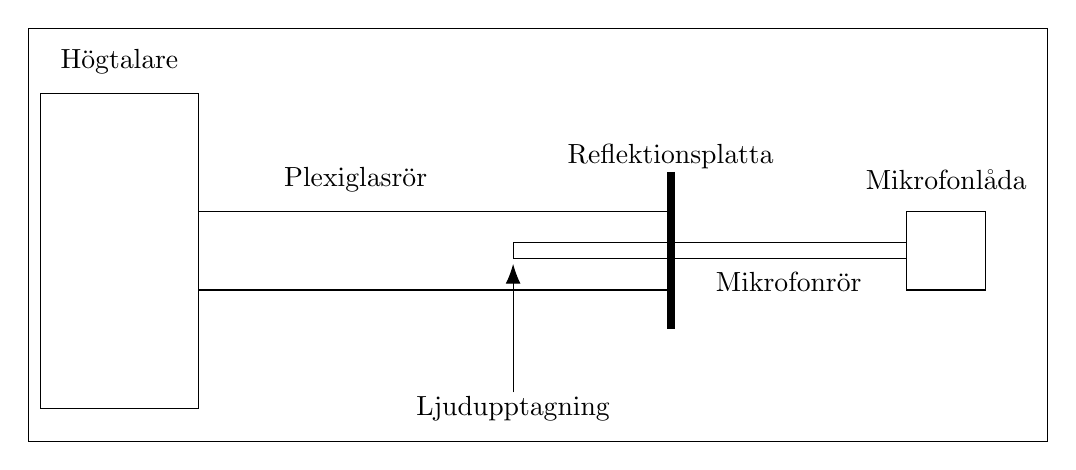
\begin{tikzpicture}[framed]
  \draw [line width=1mm] (0, 1) -- (0, -1);  % reflektionsplatta
  \draw (0, 0.5) rectangle (-6, -0.5);  % plexiglasrör
  \draw (-6, 2) rectangle (-8, -2);  % högtalare
  \draw (3, 0.5) rectangle (4, -0.5);  % mikrofonlåda
  \draw (3, 0.1) rectangle (-2, -0.1);  % mikrofonrör
  \node at (-7, 2.4) {Högtalare};
  \node at (-4, 0.9) {Plexiglasrör};
  \node at (-2, -2) {Ljudupptagning};
  \node at (3.5, 0.9) {Mikrofonlåda};
  \node at (1.5, -0.4) {Mikrofonrör};
  \node at (0, 1.2) {Reflektionsplatta};
  \draw [-{Latex[length=2.5mm]}] (-2, -1.8) -- (-2, -0.168);  % ja, decimalerna behövs
\end{tikzpicture}
\caption{Experimentuppställning --- del 1}%
\label{fig:uppställning_1}
\end{figure}

\begin{displayquote}
En högtalare är tätt ansluten till ena änden av ett grovt plexiglasrör med ca 5
cm diameter. Från högtalaren sänds en ljudvåg axiellt in i röret, som kommer att
fungera som en ljudledare. I den andra änden kan en reflektor i form av en
metallplatta anslutas tätt till röret. Ljudvågen reflekteras mycket bra mot
metallplattan och i röret uppstår det då en samverkan mellan två motriktade
vågor, som har i stort sett samma amplitud. Genom ett litet hål i reflektorn kan
ett smalt rör föras axiellt i det grova röret. Det smala röret blir också en
ljudledare och leder ljudet från änden inne i det stora röret till den yttre
änden utanför reflektorn. Den yttre änden är ansluten till en tryckmätande
mikrofon, som alltså registrerar vad som händer inne i det grova röret just där
det smala röret mynnar. Mikrofonen är i sin tur ansluten till ett oscilloskop
som visar ljudsvängningarna inne i det grova röret.
\end{displayquote}

% förklara oscilloskopet

\emph{Undersök om det är en tryckbuk eller en trycknod precis i änden på det
  grova röret. Hur kan detta förklaras fysikaliskt?}

Precis vid reflektionsplattan visade oscilloskopet en sinusvåg med hög amplitud,
vilket betyder att vi mätte en tryckbuk. % förklara fysikaliskt

\emph{Beräkna ljudhastigheten med hjälp av $v = \lambda f$ för några olika $f$}.

\begin{table}[h]
  \begin{tabular}{|l|l|l|l|} \hline
    \bfseries Frekvens & \bfseries Våglängd & \bfseries Ljudhastighet \\\hline
    \SI{1000}{\hertz} & \SI{0.344}{\meter} & \SI{344}{\meter\per\second} \\\hline
    \SI{1500}{\hertz} & \SI{0.228}{\meter} & \SI{343}{\meter\per\second} \\\hline
    \SI{2000}{\hertz} & \SI{0.174}{\meter} & \SI{348}{\meter\per\second} \\\hline
    \SI{2500}{\hertz} & \SI{0.140}{\meter} & \SI{350}{\meter\per\second} \\\hline
  \end{tabular}
\end{table}

\emph{Beräkna värdet på ljudhastigheten med följande teoretiska uttryck och
  givna värden. Hur stor är den relativa avvikelsen mellan de beräknade och
  uppmätta ljudhastigheterna?}

\begin{equation*}
  v = \sqrt{\frac{\gamma R T}{M}}
\end{equation*}

$\gamma = \num{1.40}$ \\ $M = \SI{0.0289}{\kilogram\per\mol}$ \\
$R = \SI{8.314}{\joule\per\mol\per\kelvin}$.

$T$ uppmättes till
$\SI[scientific-notation=false]{21.8}{\celsius} = \SI[scientific-notation=false]{294.95}{\kelvin}$
vilket ger en teoretisk ljudhastighet på
\SI[scientific-notation=false]{344.6}{\meter\per\second}. % TODO avg and avvikelse

\emph{Placera en absorbent i röret mot metallreflektorn och mät abosrptionen för
några olika frekvenser. Skissa ett diagram mot $\alpha$ mot $f$ utifrån
mätningarna.}

\begin{figure}[h]
  \centering
  \begin{tikzpicture}
    \begin{axis} [
      ylabel=$\alpha$,
      xlabel=$f$ (\si{\hertz}),
      xmin=0, xmax=2800,
      ymin=0, ymax=0.5,
      ]
      \addplot+ [only marks] table [col sep=comma, x index=0, y index=1] {f_alpha.dat};
    \end{axis}
  \end{tikzpicture}
  \caption{$\alpha$ beroende av $f$}%
  \label{fig:f_alpha}
\end{figure}

\emph{Välj en frekvens på ca 1,5 kHz och variera absorbentens avstånd från
  reflektorn. Mät $\alpha$ för några olika avstånd och skissa ett diagram
  utifrån mätningarna.}

\begin{figure}[h]
  \centering
  \begin{tikzpicture}
    \begin{axis} [
      ylabel=$\alpha$,
      xlabel=$x$ (\si{\meter}),
      xticklabel style={
            /pgf/number format/fixed,
            /pgf/number format/precision=2,
            /pgf/number format/fixed zerofill
      },
      ymin=0,
      ]
      \addplot+ [only marks] table [col sep=comma, x index=0, y index=1] {x_alpha.dat};
    \end{axis}
  \end{tikzpicture}
  \caption{$\alpha$ beroende av $x$}%
  \label{fig:f_alpha}
\end{figure}


För mätningar mellan $0$ och \SI[scientific-notation=false]{10}{\centi\meter}
syntes ett lokalt maximum vid $x=\SI[scientific-notation=false]{6}{\centi\meter}$.

\emph{Hur stort är avståndet med maximal absorption uttryckt i våglängder?
  Förklara varför det är maximal absorption vid den positionen.}

Maximal absorption skedde i närheten av $x=\frac{\lambda}{4}$. Vid det avståndet
sker maximal partikelrörelse (eftersom det vid $x=\frac{\lambda}{2}$, precis
som vid $x=0$, sker minimal partikelrörelse), vilket betyder att ``mer'' energi
kan överföras till absorbenten och bli värme via friktion.

\section{Vibrerande sträng}

\begin{displayquote}
På labbplatsen finns en enkel version av en ``diddley bow'' vilket i princip
består av en bräda med två upphöjningar med en uppspänd sträng emellan. Det här
är ett mycket enkelt instrument men man kan få det att låta rätt kul.

Det är även en lämplig uppställning för att illustrera olika egenskaper hos
stående vågor och stränginstrument. I försöksuppställningen kan spänningen i
strängen varieras med hjälp av en vikt som hängs upp i strängens ena ände. För att
ta upp vibrationerna från strängen finns det en flyttbar gitarrpickup kopplad
till ett ljudkort och en dator. Med hjälp av datorns mjukvara kan vi studera
frekvensinnehållet i signalen.
\end{displayquote}

\emph{Mät strängens massa per längdenhet med hjälp av våg och måttband. Montera
  strängen och väg upp en vikt på ca 4-7 kg och placera den på hållaren för att
  spänna strängen. Beräkna frekvensen för grundtonen utifrån ekvationen för
  vågfarten (nedan) där $T$ är spänningen i Newton och $\mu$ är strängens massa
  per längdenhet.}

\begin{equation*}
  v = \sqrt{\frac{T}{\mu}} \approx \SI[scientific-notation=false]{71}{\hertz}
\end{equation*}

\emph{Använd programmet för att läsa av frekvensen på grundtonen genom att
  placera musmarkören på grundtonens frekvenstopp. Ligger den uppmätta
  frekvensen ungefär inom förväntad felmarginal med tanke på hur noggrant vi kan
  mäta ingående variabler? (Gör ingen detaljerad felanalys, resonera utifrån att
  antalet värdesiffror bör överensstämma.)}

I programmet var det svårt att avläsa mer än att grundtonen låg någonstans
mellan $70$ och \SI[scientific-notation=false]{75}{\hertz}.

\emph{Justera programmet så att du kan se frekvensområdet 0-3 kHz. Slå an
  strängen och studera övertonerna. Är alla övertoners frekvenser multiplar av
  grundtonen?}

Ja, såvitt vi kan se.

\emph{Studera hur energin vid de olika frekvenserna avtar med tiden. Hur ser den
  generella trenden för hur snabbt de olika övertonerna dämpas vid olika
  frekvenser ut?}

Generellt avtar högre övertoner (övertoner med högre frekvens) snabbare än
övertoner med lägre frekvens.

\emph{Troligen går det att hitta övertoner som dämpas betydligt snabbare eller
  långsammare än närliggande övertoner. Försök förklara detta.}

Vissa övertoner matchar resonansfrekvenser i till exempel bordet.
Ljudvibrationerna finns fortfarande kvar i det ``större'' systemet men sprids ut
över resonansobjektet med vibrationer som pickupen inte kan plocka upp.

\emph{Genom att mycket lätt röra vid strängen med fingret går det att släcka ut
  övertoner med en buk vid beröringspunkten. Var skall vi dämpa strängen för att
  släcka ut alla övertoner förutom den tredje övertonen och multiplar av den?}

För att undvika att släcka ut en ton behöver vi beröra strängen vid tonens buk.
Förutom vid ändarna, där alla toner har en buk, har första övertonen en buk vid
$x=\frac{L}{2}$, andra övertonen vid $x=\frac{L}{3}$ och tredje övertonen vid
$x=\frac{L}{4}$.

\end{document}
